\begin{blocksection}
\question Fill in each blank in the code example below so that its environment diagram is the following. You do not need to use all the blanks.

\begin{multicols}{2}
\begin{lstlisting}
def among(green):
    def us(yellow):
        _________________
        yellow += _______
        green += ________
        _________________
        return __________
    return ______________
vote = among('Red')('Blue')()
\end{lstlisting}

\columnbreak
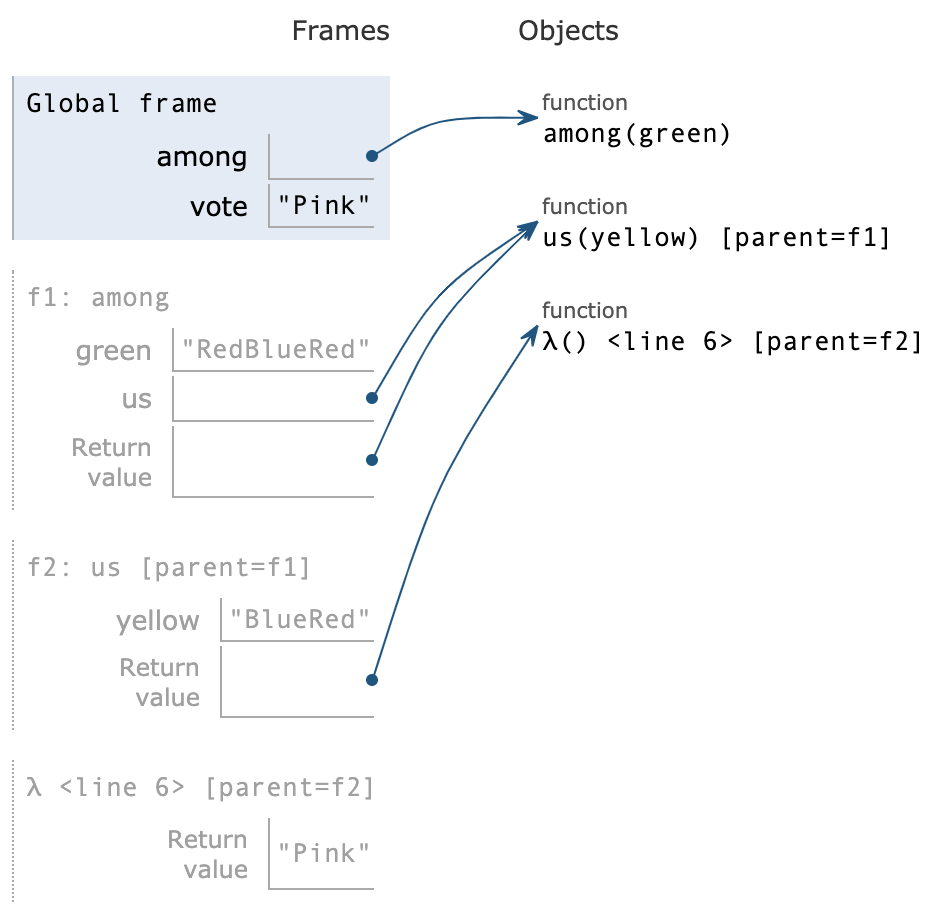
\includegraphics[width=.45\textwidth]{reverse_test.png}
\end{multicols}

\begin{solution}[2in]
\begin{lstlisting}
def among(green):
    def us(yellow):
        nonlocal green
        yellow += green
        green += yellow
        return lambda : 'Pink'
    return us
vote = among('Red')('Blue')()
\end{lstlisting}
\end{solution}
\end{blocksection}
